\section{Monte Carlo Methods}\label{sec:Monte_Carlo}

While Kalman-based extensions can alleviate some of the limitations of the original Kalman filter, they all enforce the PDF to be Gaussian at each time step. This assumption is often violated in practice, as navigation problems frequently involve highly non-linear and non-injective functions. In turn, these functions induce multimodal or heavy-tailed distributions, which cannot be adequately characterised by Gaussian hypotheses.

Monte Carlo (MC) methods \cite{bib:Metropolis,bib:SOD333-MC} offer an alternative approach that remains consistent under very mild assumptions. Their accuracy improves asymptotically with the number of samples, at the expense of an increased computational cost. This section introduces the main concepts for MC-based algorithms to solve the navigation problem \eqref{eq:navigation_problem}.

\subsection{Monte Carlo Integration}

Even though MC methods originally stem from the computation of expectations, they approximate the entire distribution \cite{bib:MC-integration}, from which every estimator of \cref{sec:state_estimation} can be derived. Being itself an expectation, the MMSE estimator is simply the most immediate, and is where we begin.

Let $X$ be a random variable taking values in $\mathbb{R}^{d_x}$ with probability density $p$, and let $\varphi\in\mathcal{L}^0(\mathbb{R}^{d_x},\mathbb{R}^{d_{\varphi}})$ such that $\varphi(X)\in\mathcal{L}^1(\mathbb{R}^{d_{\varphi}})$. We wish to compute the expectation of $\varphi(X)$:
\begin{equation}
	\mathbb{E}_p[\varphi(X)]=\int{\varphi(x)\:p(x)\:dx}\label{eq:varphi_expectation_p}
\end{equation}

Let $\mu(dx)\triangleq p(x)\:dx$ be the probability measure with density $p$ with respect to the Lebesgue measure. \eqref{eq:varphi_expectation_p} can be rewritten as:
\begin{equation}
	\langle\mu,\varphi\rangle\triangleq\int{\varphi(x)\:\mu(dx)}=\mathbb{E}_p[\varphi(X)]\label{eq:varphi_expectation_mu}
\end{equation}

Since $\mu$ is a continuous measure, evaluating \eqref{eq:varphi_expectation_mu} exactly is intractable in most practical situations. The MC method aims to approximate $\mu$ by an empirical measure induced by $N$ independent samples, as presented by \Cref{th:empirical_measure} and \Cref{th:MC_estimator}.

\begin{definition}[Empirical measure]\label{th:empirical_measure}
	Let $N\in\mathbb{N}^*$ and $X^{(1)},\dots,X^{(N)}$ be independent and identically distributed (i.i.d.) random variables drawn from $\mu$. The empirical measure associated with $\left(X^{(i)}\right)_{i\in[\![1,N]\!]}$ is defined as:
	\begin{equation}
		S^N(\mu)\triangleq\frac{1}{N}\sum_{i=1}^N\delta_{X^{(i)}}
	\end{equation}
	where $\delta_x$ denotes the Dirac measure at $x$.
\end{definition}

\begin{proposition}[Monte Carlo estimator]\label{th:MC_estimator}
	The MC estimator:
	\begin{equation}
		\left\langle S^N(\mu),\varphi\right\rangle=\frac{1}{N}\sum_{i=1}^N\langle\delta_{X^{(i)}},\varphi\rangle=\frac{1}{N}\sum_{i=1}^N\varphi\left(X^{(i)}\right)
	\end{equation}
	is unbiased and consistent:
	\begin{align}
		\mathbb{E}_p\left[\left\langle S^N(\mu),\varphi\right\rangle\right]&=\mathbb{E}_p[\varphi(X)]=\langle\mu,\varphi\rangle\\
		\left\langle S^N(\mu),\varphi\right\rangle&\overset{a.s.}{\longrightarrow}\langle\mu,\varphi\rangle
	\end{align}

	If moreover $\varphi(X)\in\mathcal{L}^2(\mathbb{R}^{d_{\varphi}})$, its mean squared error is:
	\begin{equation}
		\mathbb{E}_p\left[\left|\left\langle S^N(\mu)-\mu,\varphi\right\rangle\right|^2\right]=\frac{1}{N}\operatorname{tr}\mathbb{V}_\mu[\varphi]
	\end{equation}
	where $\mathbb{V}_\mu[\varphi]\triangleq\left\langle\mu,(\varphi-\langle\mu,\varphi\rangle)(\varphi-\langle\mu,\varphi\rangle)^\top\right\rangle$ is the covariance matrix of $\varphi$ under $\mu$, and its rescaled error converges in distribution to a centred Gaussian:
	\begin{equation}
		\sqrt{N}\left\langle S^N(\mu)-\mu,\varphi\right\rangle\overset{\mathcal{L}}{\longrightarrow}\mathcal{N}(0,\mathbb{V}_\mu[\varphi])
	\end{equation}
\end{proposition}

\begin{proof}
	By linearity of the expectation and the transfer theorem, it comes that:
	\begin{equation}
		\begin{aligned}
		\mathbb{E}_p\left[\left\langle S^N(\mu),\varphi\right\rangle\right]&=\frac{1}{N}\sum_{i=1}^N\mathbb{E}_p\left[\varphi\left(X^{(i)}\right)\right]\\
		&=\frac{1}{N}\sum_{i=1}^N\langle\mu,\varphi\rangle\\
		&=\langle\mu,\varphi\rangle
		\end{aligned}
	\end{equation}
	Furthermore, by independence of the $X^{(i)}$:
	\begin{equation}
		\begin{aligned}
		\mathbb{E}_p\left[\left|\left\langle S^N(\mu)-\mu,\varphi\right\rangle\right|^2\right]&=\mathbb{E}_p\left[\left|\frac{1}{N}\sum_{i=1}^N\left(\varphi\left(X^{(i)}\right)-\langle\mu,\varphi\rangle\right)\right|^2\right]\\
		&=\frac{1}{N^2}\sum_{i=1}^N\mathbb{E}_p\left[\left|\varphi\left(X^{(i)}\right)-\langle\mu,\varphi\rangle\right|^2\right]\\
		&=\frac{1}{N^2}\sum_{i=1}^N\mathbb{E}\left[|\varphi(X)-\langle\mu,\varphi\rangle|^2\right]\\
		&=\frac{1}{N}\operatorname{tr}\mathbb{V}_\mu[\varphi]
		\end{aligned}
	\end{equation}

	Finally, the a.s. convergence and the convergence in distribution follow respectively from the strong law of large numbers and the central limit theorem, applied to the i.i.d. variables $\varphi\left(X^{(i)}\right)$.
\end{proof}

Informally, this means that:
\begin{equation}
	S^N(\mu)=\frac{1}{N}\sum_{i=1}^N\delta_{X^{(i)}}\approx\mu
\end{equation}
in the sense that, for any measurable function $\varphi$ such that $\varphi(X)$ is integrable:
\begin{equation}
	\left\langle S^N(\mu),\varphi\right\rangle=\frac{1}{N}\sum_{i=1}^N\varphi\left(X^{(i)}\right)\approx\langle\mu,\varphi\rangle
\end{equation}

\subsection{Importance Sampling}

The standard MC method requires sampling directly from $\mu$, which can be complex in practice. Importance sampling \cite{bib:importance-sampling} circumvents this issue by drawing from a chosen importance, or proposal, distribution $\nu$ with density $q$.

Assuming that $\operatorname{supp}(q)\subseteq\operatorname{supp}(p)$, and for $x\in\operatorname{supp}(q)$, it follows from the identity $p(x)=\frac{p(x)}{q(x)}\:q(x)$ and the transfer theorem that:
\begin{equation}
	\mathbb{E}_p[\varphi(X)]=\int{\left(\varphi(x)\:\frac{p(x)}{q(x)}\right)\:q(x)\:dx}=\mathbb{E}_q\left[\varphi(X)\:\frac{p(X)}{q(X)}\right]
\end{equation}

Using measure theory notations, this is equivalent to writing:
\begin{equation}
	\langle\mu,\varphi\rangle=\left\langle\nu,\frac{d\mu}{d\nu}\:\varphi\right\rangle
\end{equation}

The density $\frac{d\mu}{d\nu}$ is known as the Radon-Nikodym derivative. This motivates the introduction of the weighted empirical measure, given by \Cref{th:weighted_empirical}.

\begin{definition}[Weighted empirical measure]\label{th:weighted_empirical}
	Let $\nu(dx)=q(x)\:dx$ with $\operatorname{supp}(\mu)\subseteq\operatorname{supp}(\nu)$, and let $X^{(1)},\dots,X^{(N)}\overset{i.i.d.}{\sim}\nu$. The associated weighted empirical measure is:
	\begin{equation}
		S^N(\mu,\nu)\triangleq\frac{d\mu}{d\nu}\:S^N(\nu)=\frac{1}{N}\sum_{i=1}^N\frac{p(X^{(i)})}{q(X^{(i)})}\:\delta_{X^{(i)}}
	\end{equation}
\end{definition}

Pairing this measure with a test function $\varphi$ yields the weighted MC estimator of \Cref{th:weighted_MC}.

\begin{proposition}[Weighted MC estimator]\label{th:weighted_MC}
	The weighted MC estimator:
	\begin{equation}
		\left\langle S^N(\mu,\nu),\varphi\right\rangle=\frac{1}{N}\sum_{i=1}^N\frac{p\left(X^{(i)}\right)}{q\left(X^{(i)}\right)}\:\varphi\left(X^{(i)}\right)
	\end{equation}
	is unbiased and consistent:
	\begin{align}
		\mathbb{E}_p\left[\left\langle S^N(\mu,\nu),\varphi\right\rangle\right]&=\mathbb{E}_p[\varphi(X)]\\
		\left\langle S^N(\mu,\nu),\varphi\right\rangle&\overset{a.s.}{\longrightarrow}\mathbb{E}_p[\varphi(X)]
	\end{align}

	Furthermore, when $\mathbb{V}_\nu\!\left[\frac{d\mu}{d\nu}\:\varphi\right]<\infty$, its mean squared error and rescaled error satisfy:
	\begin{align}
		\mathbb{E}_q\left[\left|\left\langle S^N(\mu,\nu)-\mu,\varphi\right\rangle\right|^2\right]&=\frac{1}{N}\operatorname{tr}\mathbb{V}_\nu\left[\frac{d\mu}{d\nu}\:\varphi\right]\\
		\sqrt{N}\left\langle S^N(\mu,\nu)-\mu,\varphi\right\rangle&\overset{\mathcal{L}}{\longrightarrow}\mathcal{N}\left(0,\mathbb{V}_\nu\left[\frac{d\mu}{d\nu}\:\varphi\right]\right)
	\end{align}
\end{proposition}

\begin{proof}
	This is direct using the results of \Cref{th:MC_estimator}.
\end{proof}

For $\varphi\equiv1$, the total mass:
\begin{equation}
	\left\langle S^N(\mu,\nu),1\right\rangle=\frac{1}{N}\sum_{i=1}^N\frac{p\left(X^{(i)}\right)}{q\left(X^{(i)}\right)}
\end{equation}
converges a.s. to $1$, but each finite sample is not necessarily normalised. Furthermore, $p$ and $q$ are often known only up to normalising constants $\tilde{p}=C_\mu p$ and $\tilde{q}=C_\nu q$. To alleviate these issues, \Cref{th:self_normalised_measure} introduces the self-normalised measure \cite{bib:self-normalised}, whose estimator remains consistent despite these unknown constants, as proven by \Cref{th:self_normalised_estimator}.

\begin{definition}[Self-normalised measure]\label{th:self_normalised_measure}
	Let $X^{(1)}, \dots,X^{(N)}\overset{i.i.d.}{\sim}\nu$, with $\tilde{\mu}=C_\mu\mu$ and $\tilde{\nu}=C_\nu\nu$. The self-normalised measure is:
	\begin{align}
		\tilde{S}^N(\mu,\nu)&\triangleq\sum_{i=1}^Nw^{(i)}\:\delta_{X^{(i)}}\label{eq:self_normalised_estimator}\\
		w^{(i)}&\triangleq\left.\tilde{w}^{(i)}\middle/\sum_{j=1}^N\tilde{w}^{(j)}\right.\\
		\tilde{w}^{(i)}&\triangleq\frac{\tilde{p}\left(X^{(i)}\right)}{\tilde{q}\left(X^{(i)}\right)}=\frac{d\tilde{\mu}}{d\tilde{\nu}}\left(X^{(i)}\right)
	\end{align}
\end{definition}

\begin{proposition}[Self-normalised estimator]\label{th:self_normalised_estimator}
	The self-normalised estimator:
	\begin{equation}
		\left\langle\tilde{S}^N(\mu,\nu),\varphi\right\rangle=\sum_{i=1}^Nw^{(i)}\:\varphi\left(X^{(i)}\right)=\frac{\displaystyle\left\langle S^N(\tilde{\mu},\tilde{\nu}),\varphi\right\rangle}{\displaystyle\left\langle S^N(\tilde{\mu},\tilde{\nu}),1\right\rangle}
	\end{equation}
	is biased at finite $N$, but consistent as soon as $\varphi(X)\in\mathcal{L}^1(\mathbb{R}^{d_{\varphi}})$ and $\operatorname{supp}(\mu)\subseteq\operatorname{supp}(\nu)$:
	\begin{equation}
		\left\langle\tilde{S}^N(\mu,\nu),\varphi\right\rangle\overset{a.s.}{\longrightarrow}\langle\mu,\varphi\rangle
	\end{equation}
\end{proposition}

\begin{proof}
	Although the bias of $\tilde{S}^N(\mu,\nu)$ admits no simple closed-form expression in general, it can be computed for $N=1$. In this situation, the self-normalisation forces the single weight to $1$, such that:
	\begin{equation}
		\left\langle\tilde{S}^1(\mu,\nu),\varphi\right\rangle=\varphi\left(X^{(1)}\right)
	\end{equation}
	and thus:
	\begin{equation}
		\mathbb{E}\left[\left\langle\tilde{S}^1(\mu,\nu),\varphi\right\rangle\right]=\langle\nu,\varphi\rangle\neq\langle\mu,\varphi\rangle
	\end{equation}
	in general.

	Furthermore, applying the strong law of large numbers separately to both the numerator and denominator of the self-normalised estimator yields:
	\begin{equation}
		\left\langle S^N(\tilde{\mu},\tilde{\nu}),\varphi\right\rangle=\frac{1}{N}\sum_{i=1}^N\tilde{w}^{(i)}\varphi\left(X^{(i)}\right)\overset{a.s.}{\longrightarrow}\left\langle\nu,\frac{d\tilde{\mu}}{d\tilde{\nu}}\:\varphi\right\rangle=\frac{C_\mu}{C_\nu}\:\langle\mu,\varphi\rangle
	\end{equation}
	and:
	\begin{equation}
		\left\langle S^N(\tilde{\mu},\tilde{\nu}),1\right\rangle=\frac{1}{N}\sum_{j=1}^N\tilde{w}^{(j)}\overset{a.s.}{\longrightarrow}\left\langle\nu,\frac{d\tilde{\mu}}{d\tilde{\nu}}\right\rangle=\frac{C_\mu}{C_\nu}\:\langle\mu,1\rangle=\frac{C_\mu}{C_\nu}\neq0
	\end{equation}

	Combining both expressions finally gives the desired result.
\end{proof}

\subsection{Sequential Importance Sampling}

In the filtering context, the target distribution is the joint posterior $p(\mathbf{x}_{0:k}|\mathbf{z}_{1:k})$ over the entire state trajectory. As new observations arrive, this distribution grows in dimension, making a static importance sampling approach impractical. Sequential importance sampling (SIS) \cite{bib:SMC-Bayesian,bib:intro-SMC} addresses this by updating the weights recursively rather than re-approximating the full trajectory at every time step.

\begin{assumption}[SIS hypotheses]\label{th:SIS_hypotheses}
	In addition to \Cref{th:Markov,th:observation_independence}, we assume that the proposal density of the previous state does not depend on the current observation:
	\begin{equation}
		q(\mathbf{x}_{0:k-1}|\mathbf{z}_{1:k})=q(\mathbf{x}_{0:k-1}|\mathbf{z}_{1:k-1})
	\end{equation}
\end{assumption}

This assumption enables the following factorisation:
\begin{equation}
	\begin{aligned}
	q(\mathbf{x}_{0:k}|\mathbf{z}_{1:k})&=q(x_k,\mathbf{x}_{0:k-1}|\mathbf{z}_{1:k})\\
	&=q(x_k|\mathbf{x}_{0:k-1},\mathbf{z}_{1:k})\:q(\mathbf{x}_{0:k-1}|\mathbf{z}_{1:k})\\
	&=q(x_k|\mathbf{x}_{0:k-1},\mathbf{z}_{1:k})\:q(\mathbf{x}_{0:k-1}|\mathbf{z}_{1:k-1})
	\end{aligned}
\end{equation}

While \Cref{th:SIS_hypotheses} is sufficient to derive the SIS algorithm, an additional assumption is often considered:
\begin{equation}
	q(\mathbf{x}_{0:k}|\mathbf{z}_{1:k})=q(x_k|x_{k-1},z_k)\:q(\mathbf{x}_{0:k-1}|\mathbf{z}_{1:k-1})\label{eq:simplification_q}
\end{equation}
so that a new particle $x_k^{(i)}$ can be propagated from $x_{k-1}^{(i)}$ and $z_k$ alone.

Using \Cref{th:Markov,th:observation_independence} at time $k$, the PDF factorises as:
\begin{equation}
	\begin{aligned}
		p(\mathbf{x}_{0:k}|\mathbf{z}_{1:k})&=p(\mathbf{x}_{0:k}|z_k,\mathbf{z}_{1:k-1})\\
		&=\frac{p(z_k|\mathbf{x}_{0:k},\mathbf{z}_{1:k-1})\:p(\mathbf{x}_{0:k}|\mathbf{z}_{1:k-1})}{p(z_k|\mathbf{z}_{1:k-1})}\\
		&=\frac{p(z_k|\mathbf{x}_{0:k},\mathbf{z}_{1:k-1})\:p(x_k,\mathbf{x}_{0:k-1}|\mathbf{z}_{1:k-1})}{p(z_k|\mathbf{z}_{1:k-1})}\\
		&=\frac{p(z_k|\mathbf{x}_{0:k},\mathbf{z}_{1:k-1})\:p(x_k|\mathbf{x}_{0:k-1},\mathbf{z}_{1:k-1})\:p(\mathbf{x}_{0:k-1}|\mathbf{z}_{1:k-1})}{p(z_k|\mathbf{z}_{1:k-1})}\\
		&=\frac{p(z_k|x_k)\:p(x_k|x_{k-1})\:p(\mathbf{x}_{0:k-1}|\mathbf{z}_{1:k-1})}{p(z_k|\mathbf{z}_{1:k-1})}\\
		&\propto p(z_k|x_k)\:p(x_k|x_{k-1})\:p(\mathbf{x}_{0:k-1}|\mathbf{z}_{1:k-1})
	\end{aligned}\label{eq:recursive_p}
\end{equation}

Let $\mathbf{x}_{0:k}^{(i)}$ denote the sequence $\left(x_0^{(i)},\dots,x_k^{(i)}\right)$. The recursive weight update is obtained by combining \eqref{eq:recursive_p} with \Cref{th:SIS_hypotheses}:
\begin{equation}
	\begin{aligned}
	w_k^{(i)}&\propto\frac{\tilde{p}\left(\mathbf{x}_{0:k}^{(i)}|\mathbf{z}_{1:k}\right)}{\tilde{q}\left(\mathbf{x}_{0:k}^{(i)}|\mathbf{z}_{1:k}\right)}\\
	&\propto\frac{\tilde{p}\left(z_k|x_k^{(i)}\right)\:\tilde{p}\left(x_k^{(i)}|x_{k-1}^{(i)}\right)\:\tilde{p}\left(\mathbf{x}_{0:k-1}^{(i)}|\mathbf{z}_{1:k-1}\right)}{\tilde{q}\left(x_k^{(i)}|\mathbf{x}_{0:k-1}^{(i)},\mathbf{z}_{1:k}\right)\:\tilde{q}\left(\mathbf{x}_{0:k-1}^{(i)}|\mathbf{z}_{1:k-1}\right)}\\
	&\propto w_{k-1}^{(i)}\:\frac{\tilde{p}\left(z_k|x_k^{(i)}\right)\:\tilde{p}\left(x_k^{(i)}|x_{k-1}^{(i)}\right)}{\tilde{q}\left(x_k^{(i)}|\mathbf{x}_{0:k-1}^{(i)},\mathbf{z}_{1:k}\right)}
	\end{aligned}\label{eq:weight_update}
\end{equation}
with the further simplification under the hypothesis of \eqref{eq:simplification_q}:
\begin{equation}
	w_k^{(i)}\propto w_{k-1}^{(i)}\:\frac{\tilde{p}\left(z_k|x_k^{(i)}\right)\:\tilde{p}\left(x_k^{(i)}|x_{k-1}^{(i)}\right)}{\tilde{q}\left(x_k^{(i)}|x_{k-1}^{(i)},z_k\right)}
\end{equation}

While the current formulation allows us to approximate the density of the full trajectory $p(\mathbf{x}_{0:k}|\mathbf{z}_{1:k})$ through the self-normalised measure of \Cref{th:self_normalised_measure}, we often only want to estimate the current state $x_k$. This can be done naturally by letting $\pi_k$ denote the projection of a $(k+1)$-tuple onto its last element:
\begin{equation}
	\pi_k:\left\{\begin{aligned}
	\left(\mathbb{R}^{d_x}\right)^{k+1}&\to\mathbb{R}^{d_x}\\
	(x_0,\dots,x_k)&\mapsto x_k
	\end{aligned}\right.
\end{equation}
and computing the self-normalised estimator for $\varphi=\pi_k$, which approximates the MMSE estimator of \cref{sec:state_estimation}:
\begin{equation}
	\hat{x}_k\triangleq\left\langle\tilde{S}^N(\mu_k,\nu_k),\pi_k\right\rangle=\sum_{i=1}^Nw_k^{(i)}\:x_k^{(i)}\approx\mathbb{E}_{p(\cdot|\mathbf{z}_{1:k})}[x_k]
\end{equation}
where $\mu_k(dx)\triangleq\tilde{p}(\mathbf{x}_{0:k}|\mathbf{z}_{1:k})\:dx$ and $\nu_k(dx)\triangleq\tilde{q}(\mathbf{x}_{0:k}|\mathbf{z}_{1:k})\:dx$. The corresponding empirical covariance matrix is:
\begin{equation}
	\hat{P}_k\triangleq\sum_{i=1}^Nw_k^{(i)}\left(x_k^{(i)}-\hat{x}_k\right)\left(x_k^{(i)}-\hat{x}_k\right)^\top
\end{equation}

The other estimators of \cref{sec:state_estimation} remain accessible, though they are not as immediate:
\begin{itemize}
	\item For a scalar state, the MMAE estimator only requires the cumulative distribution function, which $\tilde{S}^N(\mu_k,\nu_k)$ does define, and is obtained by accumulating the weights of the sorted particles until the total exceeds $\frac{1}{2}$. Its extension to a vector state is however not straightforward.
	\item The MAP estimator, on the other hand, calls for a density, which the particle approximation does not possess. In particular, $\hat{\psi}_{\mathrm{MAP}}(\mathbf{z}_{1:k})$ cannot be computed using the weights, since they are importance ratios rather than density values. The heaviest particle maximises the Radon-Nikodym derivative rather than the PDF itself, and maximising $\tilde{p}(\mathbf{x}_{0:k}|\mathbf{z}_{1:k})$ over the particles only locates a mode among the sampled locations.
\end{itemize}

As for the optimal and Kalman filters, the SIS algorithm follows the prediction/correction loop. The prediction step corresponds to the sampling of the new particle set through the proposal density, and is often called particle propagation. Conversely, the correction step is the weight update of \eqref{eq:weight_update}. The SIS algorithm is given by \Cref{alg:SIS}.

\begin{algorithm}[!htb]
	\begin{algorithmic}
	\State{$\forall i\in[\![1,N]\!],\:x_k^{(i)}\sim q\left(\cdot|x_{k-1}^{(i)},z_k\right)$}\Comment{Particle propagation}
	\State{$\forall i\in[\![1,N]\!],\:\tilde{w}_k^{(i)}=w_{k-1}^{(i)}\:\dfrac{\tilde{p}\left(z_k|x_k^{(i)}\right)\:\tilde{p}\left(x_k^{(i)}|x_{k-1}^{(i)}\right)}{\tilde{q}\left(x_k^{(i)}|\mathbf{x}_{0:k-1}^{(i)},\mathbf{z}_{1:k}\right)}$}\Comment{Weight update}
	\State{$\displaystyle\forall i\in[\![1,N]\!],\:w_k^{(i)}=\left.\tilde{w}_k^{(i)}\middle/\sum_{j=1}^N\tilde{w}_k^{(j)}\right.$}\Comment{Normalisation}
	\end{algorithmic}\caption{Sequential Importance Sampling}\label{alg:SIS}
\end{algorithm}

\begin{remark}[Feynman-Kac distribution]
	The recurrence \eqref{eq:recursive_p} can be expanded:
	\begin{equation}
		p(\mathbf{x}_{0:k}|\mathbf{z}_{1:k})\propto p(x_0)\prod_{j=1}^kp(x_j|x_{j-1})\times\prod_{j=1}^kp(z_j|x_j)
	\end{equation}
	to show that the PDF is a Feynman-Kac distribution \cite{bib:Feynman-Kac,bib:SOD333-FK}, with the transitions $p(x_j|x_{j-1})$ acting as the mutation and the likelihoods $p(z_j|x_j)$ as the selection function. Rather than being an artifice used to cancel the unknown constants, the self-normalisation introduced in \Cref{th:self_normalised_measure} is thus, more fundamentally, the normalisation of this distribution.
\end{remark}

\subsubsection{Numerical correction of the covariance matrix}

For numerical reasons, the estimated covariance matrix $\hat{P}_k$ may not satisfy SPD properties in practice. While an analytic reformulation existed for the Kalman filter, the numerical nature of MC methods prevents a similar solution. Formally, we want to find the closest matrix $M_+^*\succ0$ to $\hat{P}_k$ in the sense of the Frobenius norm:
\begin{equation}
	A\in\mathcal{M}_{d_x,d_x}(\mathbb{R})\mapsto\|A\|_F\triangleq\sqrt{\sum_{i=1}^{d_x}\sum_{j=1}^{d_x}{A_{i,j}}^2}
\end{equation}

If $d_x=1$, the positive real $m_+\in\mathbb{R}_+$ closest to some real $m\in\mathbb{R}$ is:
\begin{equation}
	m_+=\frac{m+|m|}{2}
\end{equation}

While this only applies to scalars, a similar operation can be performed in higher dimensions by using the SPSD term of the polar decomposition. The singular values decomposition is used to simplify the computation of the polar decomposition.

Formally, the correction algorithm \cite{bib:nearest-SPD} is as follows:
\begin{itemize}
	\item Symmetrisation of $\hat{P}_k$: $M\triangleq\dfrac{\hat{P}_k+\hat{P}_k^\top}{2}$
	\item Singular values decomposition: $M=UDV^\top$
	\item Polar decomposition: $M=\Omega\:\Sigma$ with $\Omega\triangleq U\:V^\top$ and $\Sigma\triangleq V\:D\:V^\top$
	\item Computation of $M_+$: $M_+\triangleq\dfrac{M+\Sigma}{2}$
\end{itemize}

With this algorithm, $M_+$ is ensured to be SPSD. However, we wish to achieve strict positive definiteness. To solve this issue, we recall that a symmetric matrix is SPD if and only if all its eigenvalues are strictly positive, and we introduce a small correction $\varepsilon>0$. Let $\lambda_{\min}$ denote the smallest eigenvalue of $M_+$. Let:
\begin{equation}
	\delta\triangleq\max(0,-\lambda_{\min})+\varepsilon
\end{equation}
where the first term is introduced to compensate any numerical errors introduced during the symmetrisation and SVD steps.

Since $M_+$ and $\delta I$ commute, they are simultaneously diagonalisable, and the eigenvalues of:
\begin{equation}
	M_+^*\triangleq M_++\delta I
\end{equation}
are thus:
\begin{equation}
	\lambda_i(M_+^*)=\lambda_i(M_+)+\delta\geq\lambda_{\min}+\delta>0
\end{equation}

For small enough values of $\varepsilon$, $M_+^*$ is the desired matrix.

\subsection{Weight Degeneracy}

A fundamental limitation of SIS is that the variance of the importance weights accumulates along the trajectory \cite{bib:sequential-imputations} as shown by \Cref{th:variance_weights}.

\begin{proposition}[Weight degeneracy]\label{th:variance_weights}
	Let $\mathbf{x}_{0:k}\sim\nu_k$, and let $\tilde{w}_k$ denote the non-normalised weight associated with the entire trajectory:
	\begin{equation}
		\tilde{w}_k\triangleq\frac{\tilde{p}(\mathbf{x}_{0:k}|\mathbf{z}_{1:k})}{\tilde{q}(\mathbf{x}_{0:k}|\mathbf{z}_{1:k})}
	\end{equation}

	Its variance decomposes as:
	\begin{equation}
		\mathbb{V}_{\nu_k}\left[\tilde{w}_k\right]=\mathbb{E}_{\nu_k}\left[\mathbb{V}_{\nu_k}\left[\tilde{w}_k|\mathbf{x}_{0:k-1}\right]\right]+\mathbb{V}_{\nu_k}\left[\mathbb{E}_{\nu_k}\left[\tilde{w}_k|\mathbf{x}_{0:k-1}\right]\right]\label{eq:weight_variance}
	\end{equation}
	where the first term is non-negative, and vanishes if and only if $\tilde{w}_k$ is a.s. determined by $\mathbf{x}_{0:k-1}$.
\end{proposition}

\begin{proof}
	\eqref{eq:weight_variance} is the law of total variance. Being the expectation of a non-negative quantity, its first term vanishes if and only if $\mathbb{V}_{\nu_k}[\tilde{w}_k|\mathbf{x}_{0:k-1}]$ is a.s. zero, that is if and only if $\tilde{w}_k$ is a.s. determined by $\mathbf{x}_{0:k-1}$.
\end{proof}

Given $\mathbf{x}_{0:k-1}$, the only randomness remaining in \eqref{eq:weight_variance} is the draw of $x_k$. The inner variance measures its effect, while the inner expectation integrates it out and leaves a function of $\mathbf{x}_{0:k-1}$. The first term therefore corresponds to the variance injected by $x_k$ and the second is the variance inherited from the past.

As each step adds to the previous ones, the weight distribution typically concentrates on a small number of particles, and so \eqref{eq:self_normalised_estimator} becomes a poor approximation of the PDF. While degeneracy occurs in most cases, \Cref{th:optimal_proposal} exhibits a proposal density that eliminates the additional variance introduced at the current step.

\begin{proposition}[Optimal proposal density]\label{th:optimal_proposal}
	When the proposal density is the posterior transition:
	\begin{equation}
		q(x_k|\mathbf{x}_{0:k-1},\mathbf{z}_{1:k})=p(x_k|x_{k-1},z_k)\label{eq:optimal_proposal}
	\end{equation}
	the trajectory weight is determined by $\mathbf{x}_{0:k-1}$, so that the variance introduced at step $k$ vanishes:
	\begin{equation}
		\mathbb{V}_{\nu_k}\left[\tilde{w}_k|\mathbf{x}_{0:k-1}\right]=0
	\end{equation}
\end{proposition}

\begin{proof}
	Plugging \eqref{eq:optimal_proposal} into \eqref{eq:weight_update} yields:
	\begin{equation}
		\begin{aligned}
		\tilde{w}_k&\propto\tilde{w}_{k-1}\:\frac{\tilde{p}(z_k|x_k)\:\tilde{p}(x_k|x_{k-1})}{\tilde{q}(x_k|\mathbf{x}_{0:k-1},\mathbf{z}_{1:k})}\\
		&\propto\tilde{w}_{k-1}\:\frac{\tilde{p}(z_k|x_k)\:\tilde{p}(x_k|x_{k-1})}{\tilde{p}(x_k|x_{k-1},z_k)}\\
		&\propto\tilde{w}_{k-1}\:\frac{\tilde{p}(z_k|x_k)\:\tilde{p}(x_k|x_{k-1})}{\dfrac{\tilde{p}(z_k|x_k,x_{k-1})\:\tilde{p}(x_k|x_{k-1})}{\tilde{p}(z_k|x_{k-1})}}\\
		&\propto\tilde{w}_{k-1}\:\tilde{p}(z_k|x_{k-1})\:\frac{\tilde{p}(z_k|x_k)}{\tilde{p}(z_k|x_k,x_{k-1})}\\
		&\propto\tilde{w}_{k-1}\:\tilde{p}(z_k|x_{k-1})
		\end{aligned}
	\end{equation}

	Both factors being functions of $\mathbf{x}_{0:k-1}$ alone, $\tilde{w}_k$ is determined by the conditioning, and its conditional variance is therefore zero.
\end{proof}

Using \Cref{th:optimal_proposal}, the draw of $x_k$ thus leaves $\tilde{w}_k$ untouched, but reaches $\tilde{w}_{k+1}$ through $\tilde{p}(z_{k+1}|x_k)$. Its contribution is deferred by one step rather than suppressed, and so this density delays the degeneracy rather than completely removing it. Furthermore, sampling from the posterior transition requires computing the marginal likelihood:
\begin{equation}
	p\left(z_k|x_{k-1}^{(i)}\right)=\int{p\left(z_k|x_k^{(i)}\right)p\left(x_k^{(i)}|x_{k-1}^{(i)}\right)\:dx_k^{(i)}}
\end{equation}
which is generally intractable.

A common alternative is to use the prior, or transition, density:
\begin{equation}
	q(x_k|\mathbf{x}_{0:k-1},\mathbf{z}_{1:k})=p(x_k|x_{k-1})\label{eq:prior_proposal}
\end{equation}
which is easier to compute, but ignores the current observation during propagation.

The prior density also simplifies the weight update \eqref{eq:weight_update} to:
\begin{equation}
	w_k^{(i)}\propto w_{k-1}^{(i)}\:\tilde{p}\left(z_k|x_k^{(i)}\right)\label{eq:weight_update_prior}
\end{equation}

However, because the particles are propagated without regard to $z_k$, their incremental weight is simply the likelihood $\tilde{p}\left(z_k|x_k^{(i)}\right)$. When this likelihood is peaked, most particles land where it is negligible. Only a few particles then carry most of the weight, which causes the degeneracy to accelerate. The prior is thus a less effective proposal in highly informative observation regimes.

\subsection{Sampling Importance Resampling}

Weight degeneracy is intrinsic to SIS and worsens with time unless the proposal distribution is chosen extremely close to the optimal proposal density. The sampling importance resampling (SIR) filter \cite{bib:SIR}, also known as the bootstrap filter \cite{bib:bootstrap-filter}, mitigates this by introducing a resampling step after each weight update. Resampling replaces the weighted particle set $\left\{x_k^{(i)},w_k^{(i)}\right\}_{i=1}^N$ by an unweighted set $\left\{{x_k^*}^{(j)},1/N\right\}_{j=1}^N$ drawn according to a chosen resampling algorithm:
\begin{equation}
	\left\{{x^*_k}^{(j)}\right\}_{j=1}^N=\operatorname{Resampling}\left(\left\{x_k^{(i)},w_k^{(i)}\right\}_{i=1}^N\right)\label{eq:resampling}
\end{equation}

It also uses the transition density as proposal \eqref{eq:prior_proposal}, which further reduces \eqref{eq:weight_update_prior} to:
\begin{equation}
	w_k^{(i)}\propto\tilde{p}\left(z_k|x_k^{(i)}\right)
\end{equation}
since all weights are reset to $1/N$ after resampling. This makes the SIR applicable under very weak assumptions, only requiring the ability to sample from $p(\cdot|x_{k-1})$ and compute the likelihood $p(z_k|x_k)$. Its pseudo-code is given by \Cref{alg:SIR}.

\begin{algorithm}[!htb]
	\begin{algorithmic}
	\State{$\forall i\in[\![1,N]\!],\:x_k^{(i)}\sim p\left(\cdot|x_{k-1}^{(i)}\right)$}\Comment{Particle propagation}
	\State{$\forall i\in[\![1,N]\!],\:\tilde{w}_k^{(i)}=\tilde{p}\left(z_k|x_k^{(i)}\right)$}\Comment{Weight update}
	\State{$\displaystyle\forall i\in[\![1,N]\!],\:w_k^{(i)}=\left.\tilde{w}_k^{(i)}\middle/\sum_{j=1}^N\tilde{w}_k^{(j)}\right.$}\Comment{Normalisation}
	\State{$\left\{x_k^{(j)},w_k^{(j)},-\right\}_{j=1}^N\gets\operatorname{Resampling}\left(\left\{x_k^{(i)},w_k^{(i)}\right\}_{i=1}^N\right)$}\Comment{Resampling}
	\end{algorithmic}\caption{Sampling Importance Resampling}\label{alg:SIR}
\end{algorithm}

\subsubsection{Resampling Algorithms}

Several resampling algorithms \cite{bib:resampling-methods,bib:resampling-comparison} can be used in \eqref{eq:resampling}. We present three algorithms, which all select a new particle set from the particle approximation of the PDF:
\begin{equation}
	p(x_k|\mathbf{z}_{1:k})\:dx_k\approx\sum_{i=1}^Nw_k^{(i)}\:\delta_{x_k^{(i)}}
\end{equation}

Drawing a particle from this discrete measure amounts to drawing its index $i\in[\![1,N]\!]$ from the categorical distribution of the weights $\left(w_k^{(i)}\right)_{i\in[\![1,N]\!]}$ through its cumulative distribution function (CDF):
\begin{equation}
	\left\{\begin{aligned}
	\operatorname{cdf}_i&\triangleq\sum_{j=1}^i w_k^{(j)},&i\in[\![1,N]\!]\\
	\operatorname{cdf}_0&=0
	\end{aligned}\right.
\end{equation}

As illustrated by \Cref{fig:CDF}, a draw of $u_j\in[0,1]$ uniquely determines the new particle ${x^*_k}^{(j)}$ as the parent particle $x_k^{(i)}$ of index $i$ satisfying:
\begin{equation}
	\operatorname{cdf}_{i-1}\leq u_j<\operatorname{cdf}_i
\end{equation}

\begin{figure}[!htb]
	\centering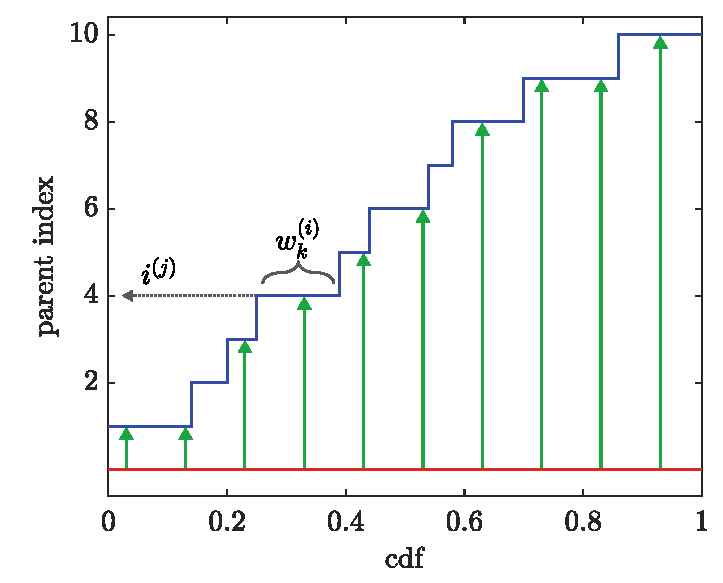
\includegraphics[width=0.7\textwidth]{../../Images/Rééchantillonnage CDF.pdf}
	\caption{An example CDF of the particle weights. The width of each step is equal to the corresponding weight, so heavier particles are more likely to be selected.}\label{fig:CDF}
\end{figure}

The main difference between the three algorithms lies in how the $N$ samples $\{u_j\}_{j\in[\![1,N]\!]}$ are generated:
\begin{itemize}
	\item\textbf{Multinomial resampling.} All the draws are independent:
	\begin{equation}
		u_j\overset{i.i.d.}{\sim}\mathcal{U}([0,1])
	\end{equation}
	This is the most natural method, but has the highest resampling variance.
	\item\textbf{Systematic or Kitagawa resampling \cite{bib:Kitagawa}.} A single draw generates all samples via:
	\begin{equation}
		\left\{\begin{aligned}
		u_1&\sim\mathcal{U}([0,1/N])\\
		u_j&=u_1+(j-1)/N,\:j\in[\![2,N]\!]
		\end{aligned}\right.
	\end{equation}
	This significantly reduces the variance of the resampling step and is generally preferred in practice.
	\item \textbf{Deterministic resampling.} All samples are deterministic such that, for some $m\in[0,1]$:
	\begin{equation}
		u_j=(j-m)/N,\:j\in[\![1,N]\!]
	\end{equation}
	This eliminates resampling variance entirely at the cost of a deterministic bias.
\end{itemize}

Some advanced filters, such as the auxiliary particle filter, presented in \cref{sec:particle_filtering}, require keeping track of the parent index $i^{(j)}$ of each resampled particle. This value is thus recorded at the creation of each new particle. \Cref{alg:Kitagawa} presents a linear implementation of the Kitagawa resampling algorithm, using the fact that both the CDF values and the Kitagawa samples are increasing to compute the parent indices sequentially.

\begin{algorithm}[!htb]
	\begin{algorithmic}
	\State{$\operatorname{cdf}_0=0$}\Comment{Computation of the CDF}
	\State{$\forall i\in[\![1,N]\!],\:\operatorname{cdf}_i=\operatorname{cdf}_{i-1}+w_k^{(i)}$\vspace{0.5\baselineskip}}
	\State{$u_1\sim\mathcal{U}([0,1/N])$}\Comment{Kitagawa samples}
	\State{$\forall j\in[\![2,N]\!],\:u_j=u_1+(j-1)/N$\vspace{0.5\baselineskip}}
	\State{$i=1$}
	\For{$j=1:N$}
	\While{$u_j\geq\operatorname{cdf}_i$}\Comment{Computation of the parent index}
	\State{$i\gets i+1$}
	\EndWhile
	\State{${x^*_k}^{(j)}=x_k^{(i)}$}\Comment{Generation of the new particle}
	\State{${w^*}_k^{(j)}=1/N$}
	\State{$i^{(j)}=i$}
	\EndFor
	\end{algorithmic}\caption{Kitagawa Resampling}\label{alg:Kitagawa}
\end{algorithm}

\begin{remark}[Loss of independence]\label{th:loss_independence}
	Because resampling duplicates particles, the resulting set is no longer independent, and the i.i.d. results of \Cref{th:MC_estimator,th:weighted_MC} no longer apply. However, the resampling is unbiased and the propagation step draws the particles independently conditionally on the past. The Feynman-Kac formalism proves \cite{bib:PF-convergence,bib:these-Oudjane} that consistency and asymptotic Gaussianity still hold in this scenario, at the price of a variance larger than in the independent case and which accumulates over time.
\end{remark}
